\selectlanguage{dutch}
\chapter*{Samenvatting}
\addcontentsline{toc}{chapter}{Samenvatting}

\refstepcounter{chapter}%
\makeatletter
\global\def\thefigure{\arabic{figure}}
%\renewcommand{\fnum@figure}{Figuur~1}
\makeatother

\bc
% dit proefschrift
Het proefschrift onderzoekt hoe \note{niet beschrijft} beschrijft het ontwerp en de architectuur van Proxima en geeft een formele specificatie van de editor. Met het prototype, ge�mplementeerd in de functionele programmeertaal Haskell, zijn al een aantal interessante editors gebouwd.
dit erbij??\ec


% documenten en editors
Een computergebruiker heeft over het algemeen te maken met een grote verscheidenheid aan documenten, zoals tekstbestanden, spreadsheets en webpagina's. De applicaties waarmee deze documenten bewerkt kunnen worden zijn zogenoemde {\em editors}, met als voorbeelden tekstverwerkers, spreadsheet-applicaties en HTML-editors. Ondanks de uiterlijke verschillen tussen editors vertonen de edit-operaties (tekst invoeren, selecteren, knippen/plakken, etc.) sterke overeenkomsten. 
% Door te abstraheren van de verschillen, kan een generieke editor ontworpen
% worden die gebruikt kan worden voor een groot aantal specifieke toepassingen. 


% wat is een generieke editor
Proxima is een generieke editor waarmee een groot aantal verschillende documenttypes bewerkt kan worden. 
Om in te zien wat een generieke editor precies is, kunnen we editen vergelijken met het maken van vruchtensap. 
%Voor een eenvoudige metafoor voor een generieke editor kunnen we kijken naar het probleem om
% van vruchten sap te maken.
Van sinaasappels, bananen en druiven kan sap gemaakt worden met een citruspers, een blender en een druivenpers. Er zijn dus drie verschillende apparaten nodig, die elk een eigen gebruiksaanwijzing hebben.
%Hiervoor zijn echter drie verschillende apparaten met drie verschillende gebruiksaanwijzingen nodig. 
Bovendien moet voor een ander soort vrucht misschien weer een nieuw apparaat aangeschaft worden. Handiger is het daarom gebruik te maken van een algemene (of generieke) sapcentrifuge, zoals de Juice Tiger$^{\text{\tiny\sf TM}}$ in Figuur~\ref{genericJuicer}. Door middel van verschillende hulpstukken kan dit apparaat sap maken van diverse soorten vruchten en zo een aantal losse apparaten vervangen.

% voordelen generiek
Zoals de sapcentrifuge een aantal losse fruitpersen vervangt, zo kan een generieke editor een aantal losse editors vervangen (zie Figuur~\ref{genericEditor}). De rol van hulpstukken wordt nu vervuld door {\em style sheets}, waarin het specifieke gedrag van de editor voor een bepaald documenttype beschreven wordt. De voordelen van een generieke editor zijn vergelijkbaar met die van de sapcentrifuge. In plaats van verschillende applicaties is er bijvoorbeeld nog maar \'e\'en applicatie, met een uniforme user interface. Het belangrijkste voordeel is echter 
dat het bouwen van een editor voor een nieuw type document met een generieke editor veel minder inspanning vergt dan op de conventionele wijze. Dit is vooral gunstig voor het bouwen van editors voor XML documenten.  

% generieke editors niet populair,
Ondanks de voordelen zijn generieke editors echter weinig populair. Om een beeld te krijgen van de reden hiervoor, werpen we eerst een wat nauwkeuriger blik op de interne structuur van een generieke editor.

%    doc en pres + editen
In de meeste editors kunnen we twee niveaus onderscheiden: het {\em  document} en de {\em presentatie}. Het document is een interne representatie van de data die door de gebruiker ge\"edit wordt. Het document is niet rechtstreeks zichtbaar, maar wordt afgebeeld op een presentatie die aan de gebruiker getoond wordt. De presentatie kan vari\"eren van platte tekst tot aan opgemaakte tekst met grafische elementen zoals lijnen en plaatjes. Het afbeelden van het document op de presentatie wordt het presentatie proces genoemd, en het weer terug afbeelden van een gewijzigde presentatie op een nieuw document het interpretatie proces.

Op het niveau van zowel het document als de presentatie zijn edit-operaties denkbaar. Een documentgerichte edit-operatie is een verandering gericht op de structuur van het document, zoals het verwisselen van twee hoofdstukken. Presentatiegerichte operaties daarentegen zijn gericht op wat er op het scherm zichtbaar is. Voor een tekstuele presentatie betekent dit dat de tekst vrij ge\"edit kan worden, zelfs als dit niet correspondeert met een edit-operatie op de structuur.

\begin{figure}
\begin{minipage}[b]{.47\textwidth}
    \begin{center}   
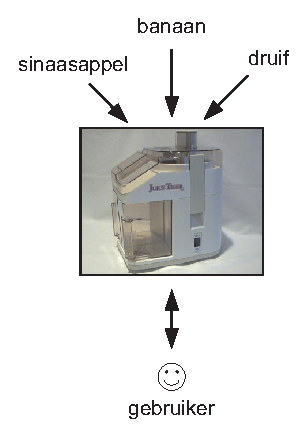
\epsfig{file=pics/eps/sapcentrifuge.eps, height=6cm}
      \caption{Een generieke sapcentrifuge.}\label{genericJuicer} 
    \end{center}
  \end{minipage}
\hfill
\begin{minipage}[b]{.47\textwidth}
    \begin{center}  
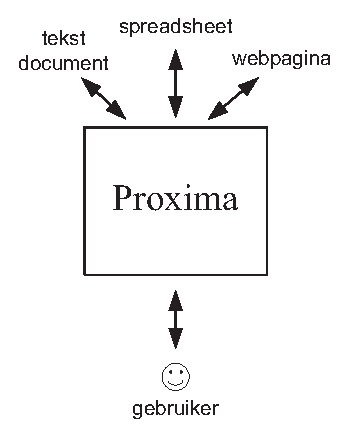
\epsfig{file=pics/eps/generiekeEditor.eps, height=6cm}
      \caption{Een generieke editor.}\label{genericEditor} 
    \end{center}
  \end{minipage}
\end{figure}


Gerelateerd aan dit onderscheid tussen edit-operaties kunnen bestaande generieke editors in twee categorie\"en ingedeeld worden. Aan de ene kant zijn er de {\em syntax-directed} editors, die een krachtig presentatiemechanisme kunnen bieden, maar vrijwel alleen documentgerichte edit-operaties bieden. Dit wordt door gebruikers vaak als beperkend  ervaren. De andere categorie wordt gevormd door de {\em syntax-recognizing} editors. Deze editors staan het vrij editen van de presentatie toe, maar beschikken weer over een beperkt presentatiemechanisme. Er bestaan ook tussenvormen ({\em hybrid} editors), maar die zijn vrijwel altijd te beschouwen als hoofdzakelijk syntax-directed danwel syntax-recognizing editors.

%Gebruiksvriendelijker zijn de presentatiegerichte generieke editors, die toestaan dat de presentatie van het %document op het scherm ge�dit kan worden. Deze editors zijn echter slechts toepasbaar voor een beperkte %klasse, veelal tekstuele, documenttypes.

\bc
generieke editors de naam gebruiksonvriendelijke applicaties te zijn met een beperkte toepasbaarheid. Een belangrijke eigenschap van Proxima is dat de editor presentatiegericht is; edit operaties kunnen worden uitgevoerd op wat op het scherm zichtbaar is, in plaats van op de interne structuur van het document. Tegelijkertijd is het ook nog steeds mogelijk om de onderliggende structuur zichtbaar te maken en te wijzigen, vergelijkbaar met het onderwaterscherm van wordperfect.
\ec


%Onderzoek hoe voordelen van documentgericht editen met presentatie gericht editen.
In dit proefschrift onderzoeken we hoe de voordelen van een generieke editor met een krachtig presentatiemechanisme te combineren zijn met een presentatiegericht edit model. 

% inventarisatie?
%Na een introductie van relevante begrippen en verschillende soorten editors in %Hoofdstuk~\ref{chap:introduction} wordt in 

Na een algemene inleiding en een introductie van relevante begrippen in Hoofdstuk~\ref{chap:introduction},
wordt in Hoofdstuk~\ref{chap:requirements} een aantal uiteenlopende toepassingen van een generieke editor beschreven.  Onder deze voorbeelden bevinden zich bekende applicaties als een editor voor programmacode, een tekstverwerker en een formule editor, maar bijvoorbeeld ook een elektronisch belastingformulier. Tezamen helpen de voorbeelden het toepassingsgebied van de Proxima editor vast te leggen. Aan de hand van de voorbeelden, die elk hun specifieke eisen stellen aan de editor, formuleren we een zestal functionele eisen, of requirements, voor een generieke editor: 
% waar een generieke editor aan zou moeten voldoen om de voorbeeld editors te kunnen implementeren:
% pres-oriented doc-oriented


%beetje afstand fruiteditor: we willen de presentatie editen. Hiervoor word het presentatie process opgesplitst %in stappen. Het terugvertalen wordt daardoor eenvoudiger. De stappen zijn gebaseerd op het presentatieproces. %niveaus (levels) lagen (layers)

\begin{description}
\item [Genericiteit.] Uitgangspunt van het onderzoek is dat de editor generiek is, en niet ontworpen voor een specifiek documenttype.
\item [Berekeningen in de presentatie.] De presentatie moet berekende waarden en structuren kunnen bevatten, zoals hoofdstuknummers en een automatische inhoudsopgave.
\item [Krachtig grafisch presentatieformalisme.] Het presentatieformalisme moet krachtig genoeg zijn om tekstverwerkingsdocumenten met wiskundige formules te tonen, maar ook  een elektronisch formulier met invoervelden en knoppen.
%A graphical presentation language with a powerful mapping formalism.]
\item [Presentatiegericht en documentgericht editen.] Edit-operaties op zowel het document als op de presentatie moeten ondersteund worden. Tevens moeten edit-operaties voor specifieke documentsoorten gespecificeerd kunnen worden.
%Niet restrictief, pres editen. Tegelijkertijd ook mogelijk om aan de hand van
% de interne structuur (bv 2 hoofdstukken verwisselen)
\item [Modeless editen.] Het moet het mogelijk zijn om eenvoudig te wisselen tussen presentatiegericht en documentgericht editen, zonder de editor expliciet in een andere toestand (mode) te moeten brengen.
%Modeless editing.]
\item [Extra state.] In sommige gevallen bevat een document informatie die niet in de presentatie zichtbaar is, en soms bevat de presentatie weer informatie die niet in het document opgeslagen is. Deze informatie noemen we {\em extra state}. De editor moet beide vormen van extra state ondersteunen.
%Support for presentation extra state as well as interpretation extra state.
\end{description}

\bc
\begin{figure}
\begin{center}
bla %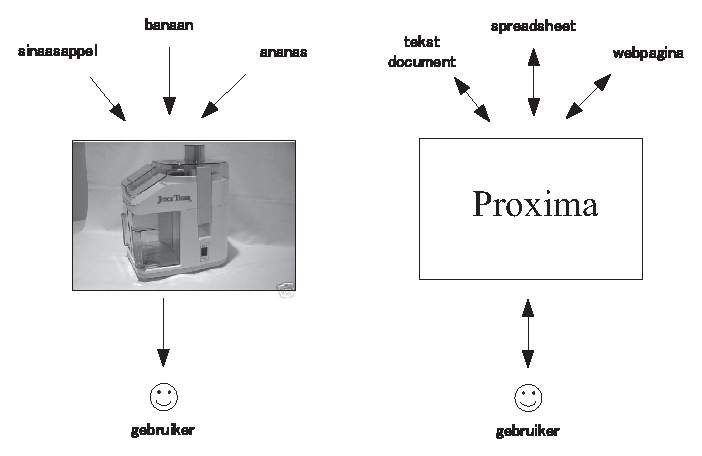
\epsfig{file=pics/eps/juicerVSeditor.eps, height=6cm}
\end{center}
\caption{Twee vormen van genericiteit.} \label{genericity}
%andere caption: Juice Tiger vs. Proxima. ?
\end{figure}
\ec



Aan de hand van bovenstaande requirements wordt een aantal bestaande systemen onder de loep genomen en met elkaar vergeleken. Het blijkt dat geen van de bestaande systemen aan alle requirements voldoet, wat betekent dat er dus geen systeem is dat alle voorbeelden kan ondersteunen. E\'en van de problemen is dat een editor aan de ene kant moet beschikken over een krachtig  presentatiemechanisme met ondersteuning voor berekende waarden, grafische elementen en eventuele duplicatie van informatie. Aan de andere kant moet voor een gebruiksvriendelijk edit model het editen van de presentatie mogelijk zijn. Dit laatste houdt echter in dat een gewijzigde presentatie terugvertaald (ge\"\i nterpreteerd) moet worden naar een nieuw document, wat moeilijker is naarmate het presentatiemechanisme complexer is. 
% en duplicaten mag bevatten

%%%%%%%%%%%%%%%% 
\bc Proxima is een presentatiegerichte editor die complexe presentaties met grafische elementen en berekende waarden ondersteunt, en daarom bruikbaar is voor een grote klasse van documenttypes.  \ec
In hoofdstuk~\ref{chap:proxArch} stellen we een gelaagde architectuur vast, voor een editor die voldoet aan de zes requirements. Het probleem om presentatiegerichte editfunctionaliteit te bieden wordt door de gelaagde architectuur opgesplitst in een aantal eenvoudigere deelproblemen. De lagen vinden hun oorsprong in het presentatie proces dat in een aantal logische stappen verdeeld kan worden. Voorbeelden van deze stappen zijn het berekenen van afgeleide waarden, het bepalen van de logische opmaak van de presentatie, tot aan het uitrekenen van alle posities en het tonen van de presentatie aan de gebruiker. Het interpretatie proces doorloopt dezelfde stappen in omgekeerde volgorde. Elk van de tussenresulaten wordt een data-niveau of {\em level} genoemd. Tussen twee niveaus bevindt zich een laag (of {\em layer}) die waarden van het ene niveau op het andere afbeeldt in zowel de presentatie als interpretatie richting.
%Eerst worden aan het document berekende waarden toegevoegd, zoals hoofdstuknummers een inhoudsopgave. Het %resultaat hiervan is de enriched document. De enriched document wordt vervolgens afgebeeld op de presentation. %Sommige documentpresentaties hebben layout informatie die niet in het document opgeslagen is (extra state), %deze wordt. Ten slotte wordt de arrangement afgebeeld op een rendering.
Het hoofdstuk geeft een overzicht van de verschillende data-niveaus en de lagen daartussen. De presentatie en interpretatie processen worden beschreven met behulp van voorbeelden. 

Hoofdstukken~\ref{chap:informalSpec} en~\ref{chap:formalSpec} geven een specificatie van de Proxima editor. Hoofdstuk~\ref{chap:informalSpec} is een inleiding op de specificatie, en geeft een model van het edit proces. Ook worden de begrippen extra state en duplicaten in de presentatie beschreven. De specificatie zelf is het onderwerp van Hoofdstuk~\ref{chap:formalSpec}. Het uitgangspunt is dat, gegeven een presentatiefunctie, een corresponderende interpretatiefunctie gespecificeerd wordt. De specificatie wordt in een aantal stappen ontwikkeld. De eerste stap is de specificatie van een editor die uit slechts \'e\'en laag bestaat en geen rekening houdt met extra state. Deze specificatie wordt vervolgens stap voor stap uitgebreid tot de specificatie van een gelaagde editor met ondersteuning voor extra state. Het hoofdstuk eindigt met een schets van de behandeling van presentaties die duplicaten kunnen bevatten.


\bc In Chapter~\ref{chap:presenting}, we discuss the {\Xprez} presentation formalism of the Proxima. {\Xprez} is a declarative presentation language, suited for specifying a wide range of presentations. We state a number of requirements for a presentation language for structured documents, and provide an informal overview of {\Xprez}, using a series of examples. \ec

Om een document af te beelden op het scherm maakt Proxima gebruik van de presentatietaal {\Xprez}. {\Xprez} is een declaratieve presentatietaal die geschikt is voor een verscheidenheid aan toepassingen. Hoofdstuk~\ref{chap:presenting} inventariseert een aantal requirements voor een presentatietaal en bevat een vergelijking van een aantal van zulke talen. Vervolgens wordt aan de hand van voorbeelden een informele beschrijving van de taal {\Xprez} gegeven.

Hoofdstuk~\ref{chap:prototype} beschrijft het prototype van Proxima, dat is ge\"\i mplementeerd in de functionele programmeertaal Haskell en voldoet aan de zes genoemde requirements. De berekende waarden en de presentatie van het document worden gespecificeerd met behulp van een attributengrammatica, terwijl de interpretatie richting met een combinator parser beschreven wordt. Het hoofdstuk toont screenshots van het prototype en bevat ook een aantal voorbeelden van de style sheets waarmee specifieke editors beschreven worden.

Ondanks de nog prille staat van het prototype is het al mogelijk om met relatief weinig moeite complexe editors te bouwen die toch prettig in het gebruik zijn. Op basis van de ervaringen met  het prototype kunnen we concluderen dat de combinatie van een krachtig presentatiemechanisme en een presentatiegericht edit model zeker mogelijk is.
% editor



\bc Even without the language support and libraries for common presentation patterns, it is already straightforward to specify a complex editor in Proxima. Thus, the Proxima prototype shows that it is possible to combine a powerful presentation formalism with a modeless integration of document-oriented and presentation-oriented editing. The resulting editors are powerful, yet easy to use.
\ec

%arch maakt het mogelijk om concise editors te specificeren die presentatie en doc combineren.

%\todo{AG}\todo{parser combinators}

\bc A prototype that offers much of the functionality discussed in this thesis has been implemented in the functional language Haskell. Chapter~\ref{chap:prototype} discusses the prototype as well as a number of editors that have been instantiated. The chapter also explains which components need to be provided to instantiate an editor. \ec

%Hoofdstuk~\ref{chap:conclusions}


\bc
Chapter~\ref{chap:requirements} explores applications of generic structure editing by providing five use cases of real-world editors. With these use cases in mind, we formulate a number of functional requirements that in our view are important for a flexible non-restrictive structure editor. We evaluate a number of existing editors according to the requirements, and conclude with an overview of how the Proxima editor is designed to meet the requirements and be able handle all use cases.

The layered architecture of Proxima is introduced in Chapter~\ref{chap:proxArch}.  The chapter discusses the various data levels, as well as the layers that maintain the mappings between the levels. The discussion is illustrated with examples of the presentation and interpretation processes.

In chapters~\ref{chap:informalSpec} and~\ref{chap:formalSpec}, we develop a specification of the Proxima editor. Chapter~\ref{chap:informalSpec} serves as an introduction to the specification and introduces our model of the edit process, as well as the concepts of extra state and duplicates in the presentation. In  Chapter~\ref{chap:formalSpec}, we start by specifying a simple editor, to which extra state and multiple layers are added in subsequent sections. The chapter ends with an informal discussion on how to handle presentations that contain duplicates.

In Chapter~\ref{chap:presenting}, we discuss the {\Xprez} presentation formalism of the Proxima. {\Xprez} is a declarative presentation language, suited for specifying a wide range of presentations. We state a number of requirements for a presentation language for structured documents, and provide an informal overview of {\Xprez}, using a series of examples.

A prototype that offers much of the functionality discussed in this thesis has been implemented in the functional language Haskell. Chapter~\ref{chap:prototype} discusses the prototype as well as a number of editors that have been instantiated. The chapter also explains which components need to be provided to instantiate an editor.

Finally, Chapter~\ref{chap:conclusions} presents the conclusions and gives an overview of future work.

\ec





%%%%%%%%%%%%%

\bc
Aanmelden Promotie

\head{Onderwerp promotieonderzoek}

Presentatiegericht editen van gestructureerde documenten en XML.

(bijvoorbeeld: 'Botontkalking bij de labrador' of 'Leerachterstand allochtone kleuters')
   
\head{Belangrijkste conclusie(s)}

Door gebruik te maken van een gelaagde architectuur is het mogelijk om een presentatiegerichte generieke editor te bouwen die geschikt is voor een breed scala aan toepassingen. 


\head{Belangrijkste aanbeveling(en)}
\ec